% Chapter 2 Part 1
\chapter{Causal Inference and Potential Outcomes}
\makeheading{Week 3}{\daterange{2022-01-17}{2022-01-21}}%chktex 8
\section{Causal Inference}
\subsection{Introduction}
\subsubsection{Reference}
\begin{itemize}
    \item Hernán M.A., \& Robins J.M. (2020). Causal Inference: What
          If. Boca Raton: Chapman Hall/CRC\@.

          \url{https://www.hsph.harvard.edu/miguel-hernan/
              causal-inference-book/}
\end{itemize}
\subsubsection{Causal Inference}
Two notions of causation:
\begin{itemize}
    \item Causes of an effect/outcome.
    \item Effects of a cause.
\end{itemize}
\textbf{Causes of an effect}
\begin{itemize}
    \item What are causes of lung cancer?
    \item What was the cause of outbreak of food poisoning?
\end{itemize}
\textbf{Effects of a cause/intervention}
\begin{itemize}
    \item Does smoking cause lung cancer?
    \item Does mixed feeding cause obesity?
    \item How strong is the effect?
\end{itemize}
\begin{itemize}
    \item We concentrate on effects of a cause/treatment/intervention.
    \item Fundamentally simpler question: search is for useful
          information rather than complete scientific understanding.
    \item Typical approach for estimating causal effects (which may be
          problematic):
          collect sample on treatments/exposures, outcomes, and other
          variables in population; Use standard statistical methods
          (such as multiple regression) to derive inferences about
          associations between observable variables.
\end{itemize}
\subsubsection*{A Note}
\begin{itemize}
    \item In pharmaceutical companies, people used to believe
          conducting randomized clinical trials is the only way to
          evaluate a newly developed drug. However, there is a shifting
          trend going on right now because of:
          \begin{itemize}
              \item Difficult to find control subjects.
              \item Compliance issue.
              \item Exclusion criteria.
              \item Cost issue.
          \end{itemize}
    \item New trend: utilizing existing Electronic Health Records data
          to help find controls.
    \item The study is not randomized any more: observational study.
\end{itemize}
\subsubsection*{Draw Causality}
\textbf{Observational Studies}
\begin{itemize}
    \item No control over which subjects have the exposure and which
          do not.
    \item Exposed and Unexposed groups may be quite different with
          respect to other subject characteristics
    \item It is sometimes useful to use these studies to look at the
          natural history of a disease, but any attempt to identify
          causality b/t a risk factor and outcome must be done w/
          great caution.
\end{itemize}
\subsection{Confounding}
\subsubsection*{Confounding Issue in Observational Studies}
\begin{Example}{}
    Differences in the outcome are not only due to the treatment, but
    also because of the masking effect of covariates (confounders).
    \begin{center}
        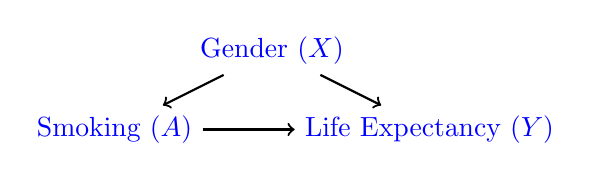
\begin{tikzpicture}[thick]
            \node (1) at (0,1) {\textcolor{Blue}{Gender ($ X $)}};
            \node (2) at (-2,0) {\textcolor{Blue}{Smoking ($ A $)}};
            \node (3) at (2,0) {\textcolor{Blue}{Life Expectancy ($ Y $)}};
            \draw[->] (1) to (2);
            \draw[->] (1) to (3);
            \draw[->] (2) to (3);
        \end{tikzpicture}
    \end{center}
    Here, gender is known as a confounder. Very often, in real
    applications, the list of potential confounders could be very large,
    and even high-dimensional.
\end{Example}
\subsubsection*{Another Example of Confounding}
\begin{Example}{}
    Researchers find when the consumption of ice cream increases, the
    death from drowning increases. Does eating ice cream lead to
    drowning?
    \begin{center}
        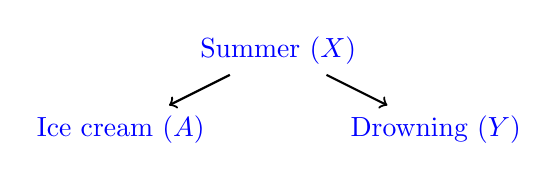
\begin{tikzpicture}[thick]
            \node (1) at (0,1) {\textcolor{Blue}{Summer ($ X $)}};
            \node (2) at (-2,0) {\textcolor{Blue}{Ice cream ($ A $)}};
            \node (3) at (2,0) {\textcolor{Blue}{Drowning ($ Y $)}};
            \draw[->] (1) to (2);
            \draw[->] (1) to (3);
        \end{tikzpicture}
    \end{center}
    Here, summer (hot weather) is a confounder.
\end{Example}
\subsubsection*{Potential Outcomes Framework}
\begin{itemize}
    \item Useful to have more precise definitions of causal effects.
    \item Demystifies the process of going from association to causation.
    \item Allows explicit statements regarding what assumptions are
          necessary to justify causal inferences.
    \item Allows for more critical, better informed evaluation of causal
          claims.
    \item Helps determine when familiar methods useful or unfamiliar
          methods necessary.
    \item Motivates derivation and use of unfamiliar methods.
\end{itemize}
\section{Potential Outcomes Framework}
\subsection*{Definition of a Causal Effect}
\begin{Regular}{}
    Suppose we have data on subjects $ i=1,\ldots,n $.
    \begin{itemize}
        \item $ \Vector{X}_i=(\Vector{X}_{i1},\Vector{X}_{i2},\ldots,\Vector{X}_{ip})^\top $: baseline covariates/potential confounders.
        \item $ A_i $: treatment assignment/exposure status for subject $ i $
              \[ A_i=\begin{cases*}
                      1, & if exposed/treated,   \\
                      0, & if unexposed/treated.
                  \end{cases*} \]
        \item $ Y_i $: observed outcome for subject $ i $.
    \end{itemize}
    \textbf{Counterfactuals/Potential outcomes}
    \begin{itemize}
        \item $ Y_i^1 $: the potential outcome if subject $ i $ were \textcolor{Blue}{treated/exposed}.
        \item $ Y_i^0 $: the potential outcome if subject $ i $ were \textcolor{Blue}{untreated/unexposed}.
    \end{itemize}
\end{Regular}
\begin{Regular}{}
    The \textbf{individual-level causal effect} for subject $ i $ is:
    \[ Y_i^1-Y_i^0. \]
\end{Regular}
\begin{Regular}{Causal Estimand}
    The \textbf{average causal effect} (ACE) is:
    \[ \ACE=\E{Y_i^1-Y_i^0}=\E{Y_i^1}-\E{Y_i^0}, \]
    where
    \begin{itemize}
        \item $ \E{Y_i^1} $ is the mean potential outcome had all subjects in the population
              were treated/exposed, and
        \item $ \E{Y_i^0} $ is the mean potential outcome had all subjects in the population were untreated/unexposed.
    \end{itemize}
    \tcblower{}
    If $ Y $ is binary,
    \begin{itemize}
        \item ACE is causal excess risk (omit subscript $ i $):
              \[ \E{Y^1-Y^0}=\E{Y^1}-\E{Y^0}=\Prob{Y^1=1}-\Prob{Y^0=1}. \]
        \item \textbf{Causal relative risk}:
              \[ \frac{\Prob{Y^1=1}}{\Prob{Y^0=1}}. \]
        \item \textbf{Causal odds ratio}:
              \[ \frac{\Prob{Y^1=1}/\Prob{Y^1=0}}{\Prob{Y^0=1}/\Prob{Y^0=0}}. \]
        \item \textbf{Crude excess risk}:
              \[ \Prob{Y=1\given A=1}-\Prob{Y=1\given A=0}. \]
        \item \textbf{Crude relative risk}:
              \[ \frac{\Prob{Y=1\given A=1}}{\Prob{Y=1\given A=0}}. \]
        \item \textbf{Crude odds ratio}:
              \[ \frac{\Prob{Y=1\given A=1}/\Prob{Y=0\given A=1}}{\Prob{Y=1\given A=0}/\Prob{Y=0\given A=0}}. \]
    \end{itemize}
\end{Regular}
\subsection*{A Toy Example}
\begin{Example}{}
    Assume we have a population of 8 subjects:
    \[ \begin{array}{cccc}
                  & A & Y^0 & Y^1 \\
            \midrule
            S_{1} & 0 & 0   & 1   \\
            S_{2} & 0 & 1   & 1   \\
            S_{3} & 0 & 0   & 0   \\
            S_{4} & 0 & 0   & 0   \\
            S_{5} & 1 & 0   & 0   \\
            S_{6} & 1 & 1   & 0   \\
            S_{7} & 1 & 1   & 1   \\
            S_{8} & 1 & 0   & 1   \\
            \bottomrule
        \end{array} \]
    We get
    \[ \text{Causal excess risk (ACE)} =\Prob{Y^1=1}-\Prob{Y^0=1}=\frac{4}{8}-\frac{3}{8}=\frac{1}{8}. \]
    For crude excess risk, we have
    \[ \begin{array}{ccccc}
                  & A & Y^0 & Y^1 & Y \\
            \midrule
            S_{1} & 0 & 0   & 1   & 0 \\
            S_{2} & 0 & 1   & 1   & 1 \\
            S_{3} & 0 & 0   & 0   & 0 \\
            S_{4} & 0 & 0   & 0   & 0 \\
            S_{5} & 1 & 0   & 0   & 0 \\
            S_{6} & 1 & 1   & 0   & 0 \\
            S_{7} & 1 & 1   & 1   & 1 \\
            S_{8} & 1 & 0   & 1   & 1 \\
            \bottomrule
        \end{array} \]
    \[ \text{Crude excess risk}=\Prob{Y=1\given A=1}-\Prob{Y=1\given A=0}=\frac{2}{4}-\frac{1}{4}=\frac{1}{4}. \]
\end{Example}
\subsection*{Fundamental Problem of Causal Inference}
\begin{Regular}{}
    For subject $ i $, we only get to observe one of $ Y_i^1 $ and $ Y_i^0 $, that is,
    \[ Y_i=Y_i^1A_i+Y_i^0(1-A_i). \]
    \tcblower{}
    \underline{Remarks}:
    \begin{enumerate}[(1)]
        \item In the literature, the above equality is often referred as the
              consistency assumption for causal inference
        \item For each subject $i$, one of the two potential outcomes is
              always missing.
        \item For this reason, many people believe causal inference is
              essentially a missing data problem.
    \end{enumerate}
\end{Regular}
\section{Estimation}
\begin{Regular}{}
    In \textbf{randomized studies}:
    \begin{itemize}
        \item $ \E{Y\given A=1}=\E{Y^1\given A=1}=\E{Y^1} $, and
        \item $ \E{Y\given A=0}=\E{Y^0\given A=0}=\E{Y^0} $.
    \end{itemize}
    Consequently, an unbiased estimate of ACE is:
    \begin{align*}
        \widehat{\ACE}
         & =\estE{Y^1}-\estE{Y^0}                                                                                   \\
         & =\estE{Y\given A=1}-\estE{Y\given A=0}                                                                   \\
         & =\frac{\sum_{i=1}^{n}Y_i A_i}{\sum_{i=1}^{n}A_i}-\frac{\sum_{i=1}^{n}Y_i(1-A_i)}{\sum_{i=1}^{n}(1-A_i)},
    \end{align*}
    where
    \begin{itemize}
        \item $ \sum_{i=1}^{n}A_i=n_1 $ is the number of treated/exposed subjects in the sample, and
        \item $ \sum_{i=1}^{n}(1-A_i)=n_0 $ is the number of untreated/unexposed subjects in the sample.
    \end{itemize}
\end{Regular}
\begin{Regular}{}
    In \textbf{observational studies}:
    \begin{itemize}
        \item $ \E{Y\given A=1}=\E{Y^1\given A=1}\ne\E{Y^1} $, and
        \item $ \E{Y\given A=0}=\E{Y^0\given A=0}\ne\E{Y^0} $,
    \end{itemize}
    where the inequalities are due to selection bias.
    Therefore, the estimator in randomized studies is biased for ACE in
    observational studies.
\end{Regular}
\section*{Assumptions for Causal Inference}
\section{Assumption 1}
\begin{Regular}{Assumption 1: Strongly Ignorable Treatment Assignment (SITA)}
    \[ (Y^0,Y^1)\indep (A\mid X). \]
    \tcblower{}
    \underline{Remarks}:
    \begin{itemize}
        \item In observational studies, it means $X$ includes all possible
              confounders (no unmeasured confounders).
        \item In randomized studies, we have $ (Y^0,Y^1)\indep A $.
        \item Within a subset of subjects with similar $X$, exposure/treatment
              can be viewed as if it were randomly assigned.
        \item This assumption cannot be verified on the observed data;
              more plausible as the size of $X$ grows.
        \item If violated, instrumental variable approach can be used in
              some cases.
    \end{itemize}
\end{Regular}
\section{Assumptions 2--4}
\begin{Regular}{Assumption 2: Stable Unit Treatment Value Assumption (SUTVA)}
    \[ (Y_i^0,Y_i^1)\indep A_j\text{ for $i\ne j$}. \]
    \tcblower{}
    \underline{Remarks}:
    \begin{itemize}
        \item Each subject's potential outcomes are not influenced by the
              actual treatment status of other subjects.
        \item Counter-example: infectious disease, family studies.
        \item If violated, divide the subjects into clusters.
    \end{itemize}
\end{Regular}
\begin{Regular}{Assumption 3: Common Support Condition (CSC)}
    \[ 0<\Prob{A=1\given X=x}<1\text{ for any $x$}. \]
    \tcblower{}
    \underline{Remarks}:
    \begin{itemize}
        \item It means that $ Y^0 $ and $ Y^1 $ should both exist in principle.
        \item Can be violated if a particular group of subjects in the
              population always receive the treatment or never receive the
              treatment.
        \item If violated, re-define the population (exclude those subjects).
    \end{itemize}
\end{Regular}
\begin{Regular}{Assumption 4: Consistency}
    \[ Y=Y^1 A+Y^0(1-A). \]
    \tcblower{}
    \underline{Remarks}:
    \begin{itemize}
        \item The observed outcome for a subject equals to the potential
              outcome under the actual treatment assignment the subject
              receives.
        \item Can be violated if different versions of treatment have
              different causal effects.
    \end{itemize}
\end{Regular}
\section{Propensity Scores}
\subsection*{Motivation for Propensity Scores}
The SITA assumption $(Y^0,Y^1)\indep (A\mid X)$ gives us some ideas about how to
estimate causal effects for observational studies.
\begin{itemize}
    \item If we condition on $X$, we can estimate the causal effect as in a
          randomized study, which is relatively straightforward.
    \item  However, if $X$ contains a large number of covariates,
          conditioning on $X$ is challenging (curse of dimensionality).
    \item  Solution: propensity score methods
\end{itemize}
\begin{Regular}{}
    \textbf{Propensity score} is the conditional probability of being exposed/treated given baseline covariates:
    \[ \ps{x}=\Prob{A=1\given X=x}. \]
    Also,
    \[ \ps{X}=\Prob{A=1\given X}. \]
    \tcblower{}
    \underline{Remarks}:
    \begin{itemize}
        \item In simple randomized studies, $ \ps{x}=0.5 $.
        \item In observational studies, $ \ps{x} $ is unknown and must be estimated.
    \end{itemize}
\end{Regular}
\subsection*{Properties}
\subsubsection*{Properties of Propensity Score}
\begin{itemize}
    \item Propensity score is a balancing score:
          \[ X\indep (A\mid \ps{X}) \]
    \item If the treatment is strongly ignorable given $ X $, that is,
          \[ (Y^0,Y^1)\indep (A\mid X), \]
          then it is strongly ignorable given $ \ps{x} $
          \[ (Y^0,Y^1)\indep (A\mid \ps{X}). \]
    \item $ \ps{x} $ is a scalar, free of dimension of $ X $.
    \item It is a summary of the contribution of all baseline characteristics to the exposure/treatment assignment.
\end{itemize}
\section{Properties of Propensity Score}
\begin{Result}{}
    The propensity score is a \textbf{balancing score}, that is,
    \[ X\indep(A\mid \ps{X}) \]
    \tcblower{}
    \textbf{Proof}: Rosenbaum and Rubin (1983).
    \begin{align*}
        \Prob[\big]{A=1\given \ps{X},X}
         & =\Prob{A=1\given X} &  & \text{$\ps{X}$ is a function of $X$} \\
         & =\ps{X}.
    \end{align*}
    On the other hand,
    \begin{align*}
        \Prob[\big]{A=1\given \ps{X}}
         & =\E[\big]{A\given \ps{X}}                                                  &  & \text{since $A$ is binary}    \\
         & =\E[\big]{\E{A\given \underbrace{X}_{C_1}}\given\underbrace{\ps{X}}_{C_2}} &  & \text{LIE since $C_2=f(C_1)$} \\
         & =\E[\big]{\ps{X}\given \ps{X}}                                                                                \\
         & =\ps{X}.
    \end{align*}
    Therefore,
    \[ \Prob[\big]{A=1\given \ps{X},X}=\Prob[\big]{A=1\given \ps{X}}. \]
    In other words, $ X\indep (A\mid \ps{X}) $.
\end{Result}
\begin{Result}{}
    If $ (Y^0,Y^1)\indep (A\mid X) $, then
    \[ (Y^0,Y^1)\indep(A\mid \ps{X}). \]
    \tcblower{}
    \textbf{Proof}:
    \begin{align*}
        \Prob{A=1\given Y^0,Y^1,\ps{X}}
         & =\E{A\given Y^0,Y^1,\ps{X}}                                                                 &  & \text{since $A$ is binary}      \\
         & =\E[\big]{\E{A\given \underbrace{Y^0,Y^1,X}_{C_1}}\given \underbrace{Y^0,Y^1,\ps{X}}_{C_2}} &  & \text{LIE since $C_2=f(C_1)$}   \\
         & =\E[\big]{\E{A\given X}\given Y^0,Y^1,\ps{X}}                                               &  & \text{SITA}                     \\
         & =\E[\big]{\ps{X}\given Y^0,Y^1,\ps{X}}                                                                                           \\
         & =\ps{X}                                                                                                                          \\
         & =\Prob[\big]{A=1\given \ps{X}}.                                                             &  & \text{from the previous result}
    \end{align*}
    Therefore,
    \[ (Y^0,Y^1)\indep(A\mid \ps{X}). \]
\end{Result}